\documentclass[a4paper]{article}

\usepackage{times}
\usepackage{tikz}
\usepackage[margin=0cm]{geometry}
\usepackage{graphicx}
\usepackage{anyfontsize}
\usepackage{fancyhdr}
\usepackage{indentfirst}
\usepackage{multicol}
\usepackage{amsmath}
\usepackage[spanish]{babel}
\usepackage[utf8]{inputenc}
\usepackage{titlesec}


\author{}
\date{}
\title{}

\begin{document}
	
	\thispagestyle{empty}
	
	\begin{tikzpicture}[remember picture, overlay]
		\pgftransformshift{\pgfpoint{0cm}{0cm}}
		%A4: 21cm x 29,7cm
		\draw [line width=2pt](1cm,-1cm) -- (1cm,-27.7cm) -- (14cm, -27.7cm) -- (14cm, -1cm) -- (1cm, -1cm);
		
		\draw[line width=2pt] (15cm, -27.7cm) -- (19cm,-27.7cm) -- (19cm, -1cm) -- (15cm, -1cm) --  (15cm, -27.7cm);
		
		\node [line width=2pt] at (17cm, -3.5cm) {
\includegraphics[width=3cm]{../imagenes/utn.png}};
		
		\node [line width=2pt] at (7.5cm, -7.5cm) {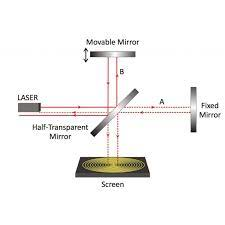
\includegraphics[width=10cm]{../imagenes/interferometro2.jpg}};
		
		\node at (17cm, -7cm) {\scalebox{5}{\textbf{U}}};
		\node at (17cm, -9cm) {\scalebox{5}{\textbf{T}}};
		\node at (17cm, -11cm) {\scalebox{5}{\textbf{N}}};
		\node at (17cm, -14cm) {\scalebox{5}{\textbf{F}}};
		\node at (17cm, -16cm) {\scalebox{5}{\textbf{R}}};
		\node at (17cm, -18cm) {\scalebox{5}{\textbf{C}}};
		
		\node at (7.5cm, -14cm) {\fontsize{16}{16}\selectfont \textbf{\textit{EL INTERFERÓMETRO}}};
		
		\node at (7.6cm, -24cm){\begin{minipage}[c]{12cm} 
			\raggedright
			\vspace{1.5cm} 
			\fontsize{14}{14}\selectfont \textbf{Autor:} Marcos Raúl Gatica\\
			\fontsize{14}{14}\selectfont \textbf{Curso:} 2R1 \\
			\fontsize{14}{14}\selectfont \textbf{Asignatura:} Física Electrónica.\\
			\fontsize{14}{14}\selectfont \textbf{Institución:} Universidad Tecnológica Nacional - Facultad Regional de Córdoba.\\
		\end{minipage}};
		
	\end{tikzpicture}
	
	%Interlineado = fuente * (valor del interlineado)
	%Ej: interlineado = 12 * (1.5) = 18 -> {12}{18}
	\renewcommand{\normalsize}{\fontsize{12}{14}\selectfont}
	\newgeometry{margin=1cm}
	
	\titleformat{\section}
		{\fontsize{12}{12}\bfseries}
		{\thesection.}{0.5em}{\underline}
	
	\pagestyle{fancy}
	\fancyhf{}
	\renewcommand{\headrulewidth}{0pt}
	\renewcommand{\footrulewidth}{0pt}
	\fancyfoot[R]{\textit{Gatica M. - Leg. 402006 - 2R1 pág. \thepage}}
	\setlength{\footskip}{0pt}
		
	\newpage
	\thispagestyle{empty}
	\text{}
	\newpage
	
	\thispagestyle{empty}
	\setcounter{page}{0}
	\tableofcontents
	
	\newpage
	\thispagestyle{fancy}
	
%	\begin{multicols}{2}
	\flushbottom
	\twocolumn
		\section{CONCEPTOS PREVIOS}
			\subsection{La interferencia}
		\indent La interferencia es un fenómeno que ocurre cuando dos o más ondas, de cualquier especie como las electromagnéticas o mecánicas, se traslapan en el espacio. Cuando esto ocurre, la onda total en cualquier punto e instante estará bajo el \textbf{principio de superposición.}
		
		\subsection{El principio de superposición}
		\indent Este principio describe cómo las ondas interactúan cuando se encuentran en el mismo espacio: \textit{"cuando dos o más ondas se interceptan en un mismo punto en el espacio, la amplitud resultante de la onda en ese punto es una suma algebraica de las amplitudes de las ondas individuales"} \newline
		
		\textbf{Ejemplo:} \newline
		\indent Dada la colisión entre dos ondas sinusoidales de la misma frecuencia y magnitud, el punto de colisión genera una onda resultante igual a:
		
		\begin{center}
			${y_1} = A.sen(kx - \omega t)$ \\ 
			${y_2} = A.sen(kx - \omega t)$ \\ \
			
			${y_{RT}} = {y_1} + {y_2}$ \\
			${y_{RT}} = 2A.sen(kx - \omega t)$ \\
		\end{center}
		
		\subsection{Interferencia constructiva y destructiva} 
		\textbf{Interferencia constructiva:}
		
		\indent Este fenómeno ocurre cuando las dos ondas están en fase, es decir, sus crestas y valles coinciden. Esto significa que las diferencias de longitud de los caminos recorridos por las ondas son múltiplos enteros de la longitud de onda $\lambda$. En el interferómetro, este caso genera franjas brillantes.
		
		\indent Matemáticamente, la interferencia constructiva existe cuando la diferencia de recorrido óptimo $\Delta L$ satisface:
		
		\begin{center}
			$\Delta L = m . \lambda$ \\
		\end{center}
		
		siendo:
		\begin{itemize}
			\item m: número entero. 
			\item $\lambda$: longitud de la luz de onda utilizada. 
			\item $\Delta L$: diferencia de recorrido entre los dos haces. \\
		\end{itemize} 
				
		\textbf{Interferencia destructiva:}
		
		\indent Este fenómeno ocurre cuando las ondas están en oposición de fase, digamos, la cresta de una onda coincide con el valle de la otra y viceversa. La diferencia de longitud de los caminos aquí es un múltiplo impar de la mitad de la longitud de onda $\lambda$/2. El resultado es una onda con amplitud mínima o nula, que genera franjas oscuras en el interferómetro.
		
		\indent La interferencia destructiva posee la siguiente condición:
		
		\begin{center}
			$\Delta L = (m . {\frac{1}{2}}) . \lambda$
		\end{center}
		
		siendo:
		\begin{itemize}
			\item m: número entero.
			\item $\lambda$: longitud de la luz de onda utilizada.
			\item $\Delta L$: diferencia de recorrido entre los dos haces.
		\end{itemize} 
		
		
		\section{EL INTERFERÓMETRO}
		
		\indent El interferómetro es un dispositivo usado para medir ondas de luz o de sonido mediante el principio de interferencia. Es usado en diversas ramas de la física para detectar pequeñas distancias, movimientos o cambios en una señal.
		
		\indent El dispositivo se usa en varios campos como la astronomía para medir el diámetro de estrellas o la distancia entre cuerpos celestes, y en la medición de ondas gravitacionales (interferómetro láser LIGO).
		
		\section {PRINCIPIO DE FUNCIONAMIENTO}
		
		\indent El interferómetro se basa en la superposición de ondas, generalmente de la luz. Este fenómeno de interferencia es el que permite detectar variaciones extremadamente pequeñas.
		
		\section{EL INTERFERÓMETRO DE MICHELSON:}
		
		\indent Es uno de los interferómetros más conocidos, su estructura básica incluye: 
		
		\begin{figure}[h!]
			\centering
			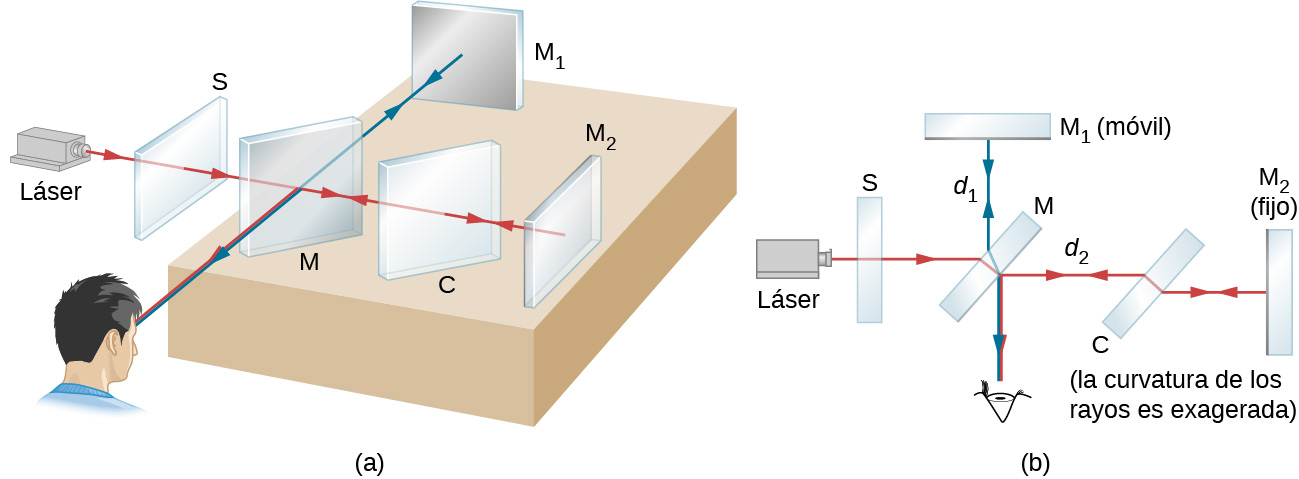
\includegraphics[width=0.4\textwidth]{../imagenes/interferometroDibujoCompleto.jpg}
			\caption{Interferómetro de Michelson - Esquema}
			\label{fig:interferometro2}
		\end{figure}
		
		\begin{enumerate}
			\item \textbf{Fuente de luz:} Se usa una luz coherente, como un láser.
			\item \textbf{Divisor de haz:} Este dispositivo divide el haz de luz en dos partes.
			\item \textbf{Espejos:} Dos espejos colocados en ángulos precisos reflejan los haces divididos.
			\item \textbf{Superposición de los haces:} Los haces de luz vuelven a unirse después de recorrer diferentes caminos, y el patrón de interferencia que se crea se observa en una pantalla o detector.
		\end{enumerate}
		
		\subsection{Matemática: Fórmula de interferencia de Michelson}
		
		El interferómetro de Michelson crea un patrón de interferencia que depende de la diferencia en la longitud de los caminos recorridos por los dos haces de luz. La fórmula para el número de franjas de interferencia observadas en el patrón es:
		
		\begin{center}
			N = $\frac{2 \Delta L}{\lambda}$ \\
		\end{center}
		
		siendo:
		\begin{itemize}
			\item N: número de franjas de interferencia.
			\item $\Delta L$: diferencia en la longitud de los caminos recorridos por los dos haces de luz.
			\item $\lambda$: longitud de onda de la luz utilizada.
		\end{itemize}
		
		\subsection{Funcionamiento}
		\begin{enumerate}
			\item \textbf{División del haz de luz:} Un haz de luz coherente, como un láser, es dividido en dos haces por un divisor.
			
			\item \textbf{Reflexión en los espejos:} Los dos haces reflejados viajan por caminos diferentes (espejos y divisor de haz) y luego se recombinan en el divisor de haz.
			
			\item \textbf{Superposición e interferencia:} Los dos haces se superponen y crean un patrón de interferencia en una pantalla o detector. La diferencia en las distancias recorridas por los haces causa una variación en el patrón de interferencia: \textbf{constructivo} si la fase es múltiplo entero de $\lambda$ o cero; \textbf{destructivo} si la diferencia de fase es múltiplo impar de $\lambda$/2.
			
			\item \textbf{Detección de desplazamientos:} Si uno de los espejos se mueve, cambiará la diferencia en las longitudes de los caminos ($\Delta L$), lo que hará variar el número de franjas de interferencia observadas. 
		\end{enumerate}
		
		\textbf{\underline{Aplicación:}} \\ \\
		\indent Dada una luz cuya longitud de onda sea de 500nm, deseamos medir la diferencia en la longitud del camino de 1micrómetro, usando la Fórmula podemos decir que:
		\begin{center}
			$N = \frac{2 \Delta L}{\lambda}$  \\ \
			\newline
			$N = \frac{2(10^{-6})}{500(10^{-9})}$  \\ \
			\newline
			$N = 4$ \\
		\end{center}
		Esto da a entender que veremos 4 franjas de interferencia moviéndose en respuesta a un cambio de 1 micrómetro en la longitud del camino.
		
		\section{EXPERIMENTO MICHELSON Y MORLEY}
		
		\indent El experimento de Michelson y Morley fue un caso de aplicación original del interferómetro desarrollado por uno de los autores. Fue esencial para el desarrollo de la teoría de la relatividad espacial de Einstein.
		
		\begin{figure}[h!]
			\centering
			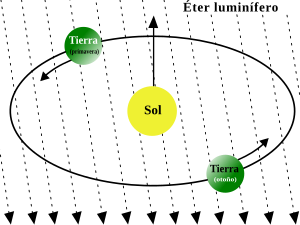
\includegraphics[width=0.189216\textwidth]{../imagenes/experimentoMM.png}
			\caption{Descripción del concepto "éter".}
			\label{fig:experimentoMM}
		\end{figure}
		
		\subsection{Contexto histórico y objetivo del experimento}
		\indent Antes de la formulación de la teoría espacial de la relatividad, los científicos creían que las ondas de luz requerían un medio de propagación, similar a las ondas mecánicas (ejemplo: ondas de sonido -> aire). Este supuesto medio lo llamaron \textbf{"éter luminífero"} y estaría presente en todo el espacio, siendo el marco de referencia para la propagación de ondas lumínicas. \newline
		\indent El objetivo del experimento era determinar la velocidad de la Tierra con respecto al éter, observando los cambios de la velocidad de la luz cuando el interferómetro de Michelson era girado en diferentes direcciones con respecto al movimiento de la Tierra. Si el planeta se movía a través del éter, se debería apreciar los cambios en la rapidez de la luz en diferentes direcciones.
		
		\subsection{Funcionamiento del experimento}
		\indent El interferómetro de Michelson dividía un haz de luz en dos, enviando las dos partes a través de trayectorias perpendiculares entre sí. Estas trayectorias recorrían distancias diferentes, lo que podía resultar en patrones de interferencia si había cambios en la velocidad de la luz a lo largo de cada trayectoria.
		\begin{itemize}
			\item \textbf{Hipótesis:} Si la Tierra se movía a través del éter, la velocidad de la luz sería diferente dependiendo de la orientación del interferómetro con respecto al movimiento del planeta. Al rotar el instrumento, los científicos esperaban observar un desplazamiento en las franjas de interferencia de $\sim$ 0,4 de una franja completa.
		\end{itemize}
		
		\subsection{Resultados}
		\indent El experimento pudo concluir en que no había desplazamiento apreciable de las franjas de interferencia, siendo menos de una centésima de franja y dentro de los límites de la incertidumbre experimental, pareciendo igual a cero. Se concluyó que no se podía detectar el movimiento de la Tierra a través del éter.
		\indent Los científicos dudaron en por qué no había un efecto en la velocidad de la luz siendo que la Tierra se movía a través del éter.
		
		\subsection{Idea clave del experimento}
		\indent La idea central es que si la luz viaja en la dirección del movimiento de la Tierra (trayectoria paralela), su velocidad relativa al observador en el planeta debería ser distinta que si viaja en dirección perpendicular. \newline
		\indent Este efecto debía causar un desfase entre los dos haces de luz en las trayectorias perpendiculares, lo que se vería como un cambio en las franjas de interferencia.\newline
		
		\textbf{Derivación del tiempo de viaje de la luz} \newline
		\indent Supongamos que el interferómetro tiene un brazo de longitud $L$, la Tierra se mueve por el éter con una velocidad $v$, y la velocidad de la luz en el vacío es $c$. \newline
		\indent Para el brazo del interferómetro alineado en la dirección del movimiento de la Tierra, el tiempo total en ir ($c-v$) y volver ($c+v$) sería:
		
		\begin{center}
			${t_{||}} = {\frac{L}{c-v}} + {\frac{L}{c+v}}$ \\ \
			\newline
			${t_{||}} = \frac{L(c+v) + L(c-v)}{(c-v)(c+v)}$ \\ \
			\newline
			${t_{||}} = \frac{cL + vL + cL - vL}{c^2 - v^2}$ \\ \
			\newline
			${t_{||}} = \frac{2cL}{c^2 - v^2}$ \\ \
			\newline
			${t_{||}} = \frac{2cL} {c^2(1 - (\frac{v}{c})^2)}$ \\ \
			\newline
			${t_{||}} = {\frac{2L}{c}} . \frac {1}{1- (\frac{v}{c})^2}$ \\ \
		\end{center}
		
		\indent Para velocidades pequeñas, como en este caso $v$ con respecto a $c$, se puede aproximar a:
		
		\begin{center}
			${t_{||}} \approx {\frac{2L}{c}} (1 + \frac{v^2}{c^2})$
		\end{center}
		
		\indent En la dirección perpendicular, el tiempo de viaje es diferente:
		\begin{figure}[h!]
			\centering
			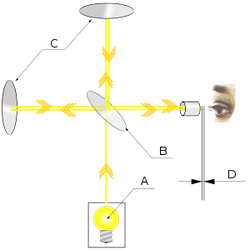
\includegraphics[width=0.15\textwidth]{../imagenes/dibujoExperimentoMM.png}
			
			
		\end{figure}
		\begin{center}
			$t_{\perp} = \frac{2L}{\sqrt{c^2 - v^2}} = {\frac{2L}{c}} \frac{1}{\sqrt{1 - \frac{v^2}{c^2}}}$  
		\end{center}
		
		\indent Como en el caso anterior, se puede hacer una aproximación dado a que $v << c$:
		
		\begin{center}
			${t_{\perp}} \approx {\frac{2L}{c}} (1 + \frac{v^2}{2c^2})$
		\end{center}
		
		\textbf{Diferencia de tiempos}
		
		\begin{center}
			$\Delta t = {t_{||}} - {t_{\perp}} = {\frac{2L}{c}} {\frac{v^2}{c^2}}$
		\end{center}
		
		\indent Este desfase era lo que Michelson y Morley esperaban ver cuando giraban el interferómetro 90º, ya que al hacerlo, la diferencia en las trayectorias debería cambiar y causar un desplazamiento en las franjas de interferencia.
		
		\subsection{Impacto en la física moderna}
		\indent En 1905 Einstein postula la teoría de la relatividad espacial, donde establece que la velocidad de la luz en el vacío es constante en todos los marcos de referencia inerciales, e independientemente de la velocidad relativa entre ellos. \newline
		\indent Con ello, se eliminaba la necesidad de un medio como el éter para la propagación de la luz.
		
%	\end{multicols}
	
\end{document}
